\documentclass[a4paper]{article}
\linespread{1.5}
\usepackage{authblk}
\usepackage[round]{natbib}
\usepackage{amssymb, amsmath}
\usepackage{url, tikz}
\usepackage{hyperref}
\usepackage[sc]{mathpazo}
\usepackage[T1]{fontenc}
\usepackage{geometry}
\geometry{verbose,tmargin=2.5cm,bmargin=2.5cm,lmargin=2.5cm,rmargin=2.5cm}
\setcounter{secnumdepth}{2}
\setcounter{tocdepth}{2}
\usepackage{url}
\usepackage[utf8]{inputenc}
\usepackage{float} 
\usepackage[nottoc]{tocbibind}

\usepackage{Sweave}
\begin{document}


\bibliographystyle{abbrvnat}

\Sconcordance{concordance:GeorgianStockParser.tex:GeorgianStockParser.Rnw:%
1 18 1 1 0 1 1 1 7 4 1 1 7 62 1 1 2 1 0 2 1 11 0 1 1 12 0 1 2 2 1 1 2 1 %
0 1 1 19 0 1 2 2 1 1 2 1 0 2 1 18 0 1 1 19 0 1 2 3 1 6 0 1 5 8 1}



\renewcommand\Authfont{\fontsize{12}{14.4}\selectfont}
\renewcommand\Affilfont{\fontsize{9}{10.8}\itshape}

\title{\textbf{Parsing Georgian Stock Market Data}}
\author{Zijie Zhu\thanks{\href{mailto:Zijie.Zhu@williams.edu}{Zijie.Zhu@williams.edu}}}
\affil{\textit{Computer Science and Statistics \\ \textit{Williams College}       \\ \textit{Williamstown, Massachusetts}\\ \textit{United States, 01267}}}
\maketitle

\setkeys{Gin}{width=0.95\textwidth}

\tableofcontents

\begin{abstract}
The \texttt{GeorgianStockParser} package provides basic tools to download data of stock market in Republic of Georgia. Basic data organizing and analyzing tools are also offered.
\end{abstract}
\newpage
\section{Introduction}
\label{sec:Introduction}

The stock market in Georgia is still much under development. Although the number of stocks and the volume of trades are still relatively small compared with developed economics, Georgian stock market will eventually grow, and it is the right time to be interested, if not investing yet, in the market. This package aims to provide a few tools to download and analyze the Georgian stock market, and be used as a data set updater.

\section{Georgian Stock Exchange Website and Data}
\label{sec:GSE}

The Georgian Stock Exchange website is still primary compared to the websites of stock exchange centers in more developed economics. On the website, there is no direct link to download the data. However, data of stock symbols and trade results are accessible after clicking into links.

\begin{figure}[H]
\centering
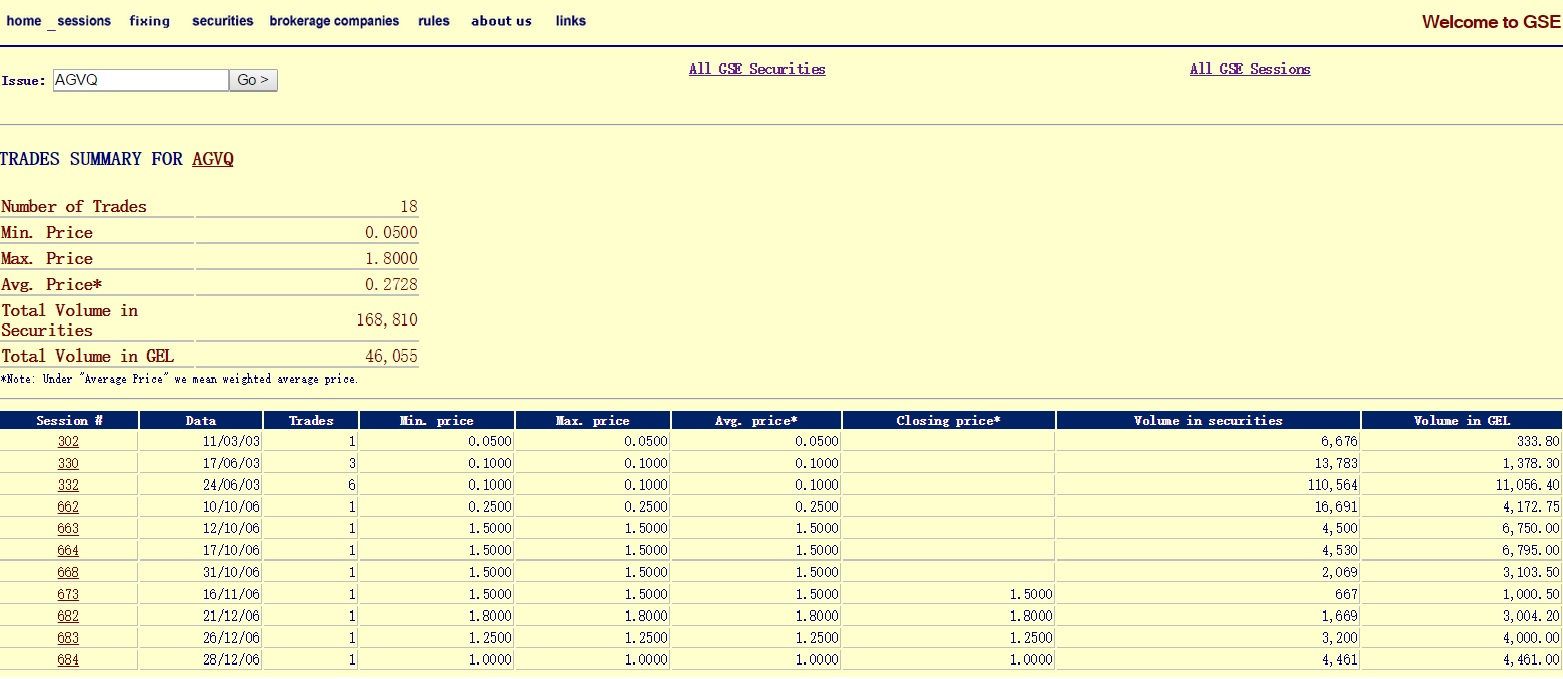
\includegraphics[width=6.3in, height=3.2in]{images/AGVQ.jpg}
\caption{GSE data taken on Jan. 14th, 2015 for Akhmeta Winery Company (stock symbol AGVQ). Information includes Session number, Date (written as ``Data'' on screenshot, probably misspelling), Trades, Min. Price, Max. Price, Avg. Price (weighted), Closing Price (weighted), Volume in Securities, and Volume in GEL (Georgian Lari). Basic summary is provided on the top-left corner. Notice that no direct download link available.}
\label{fig:AGVQ}
\end{figure}

We can also view the list of registered stock symbols.

\begin{figure}[H]
\centering
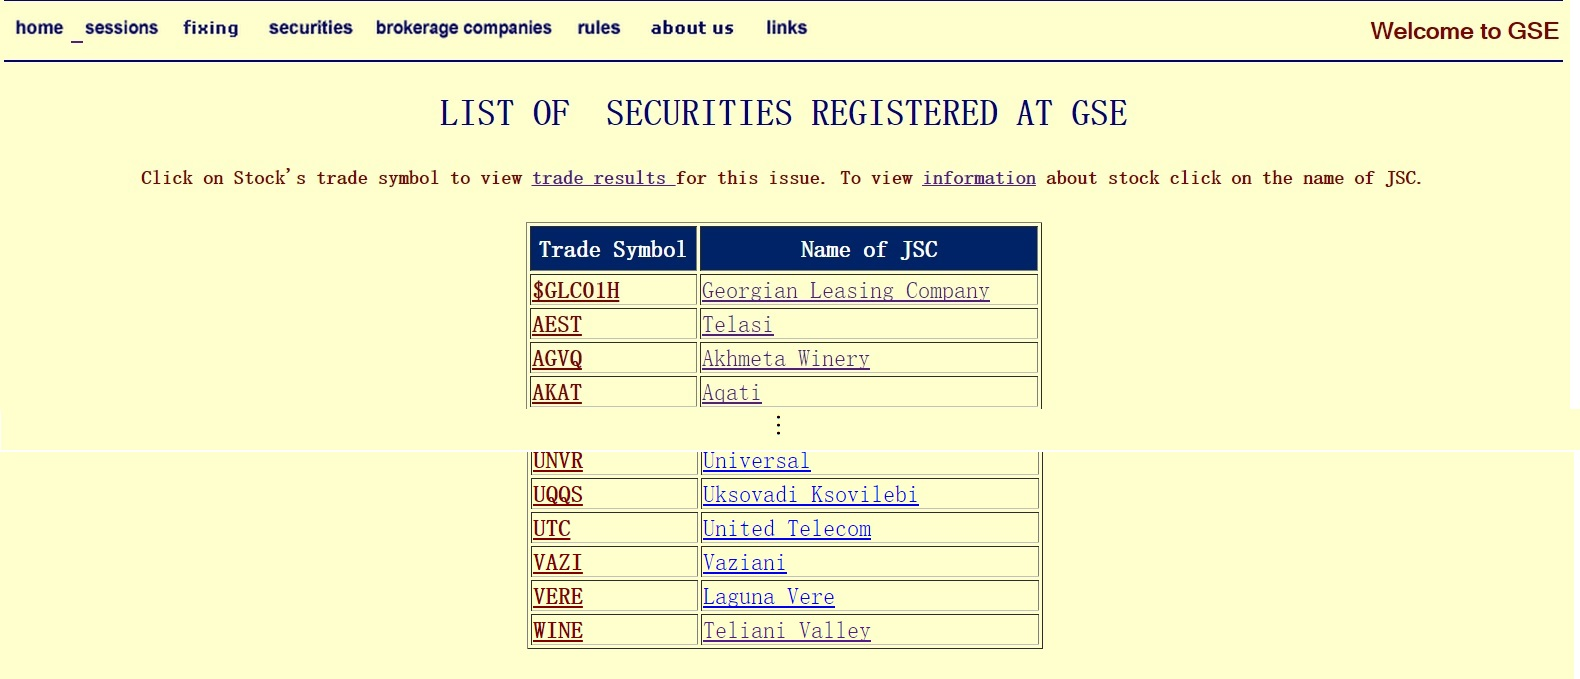
\includegraphics[width=6.3in, height=3.2in]{images/stocks.jpg}
\caption{GSE data taken on Jan. 14th, 2015 of all registered stock symbols. Notice that no direct download link available.}
\label{fig:stocks}
\end{figure}

In addition to viewing the trade result of each stock, we can view trades on every session. 

\begin{figure}[H]
\centering
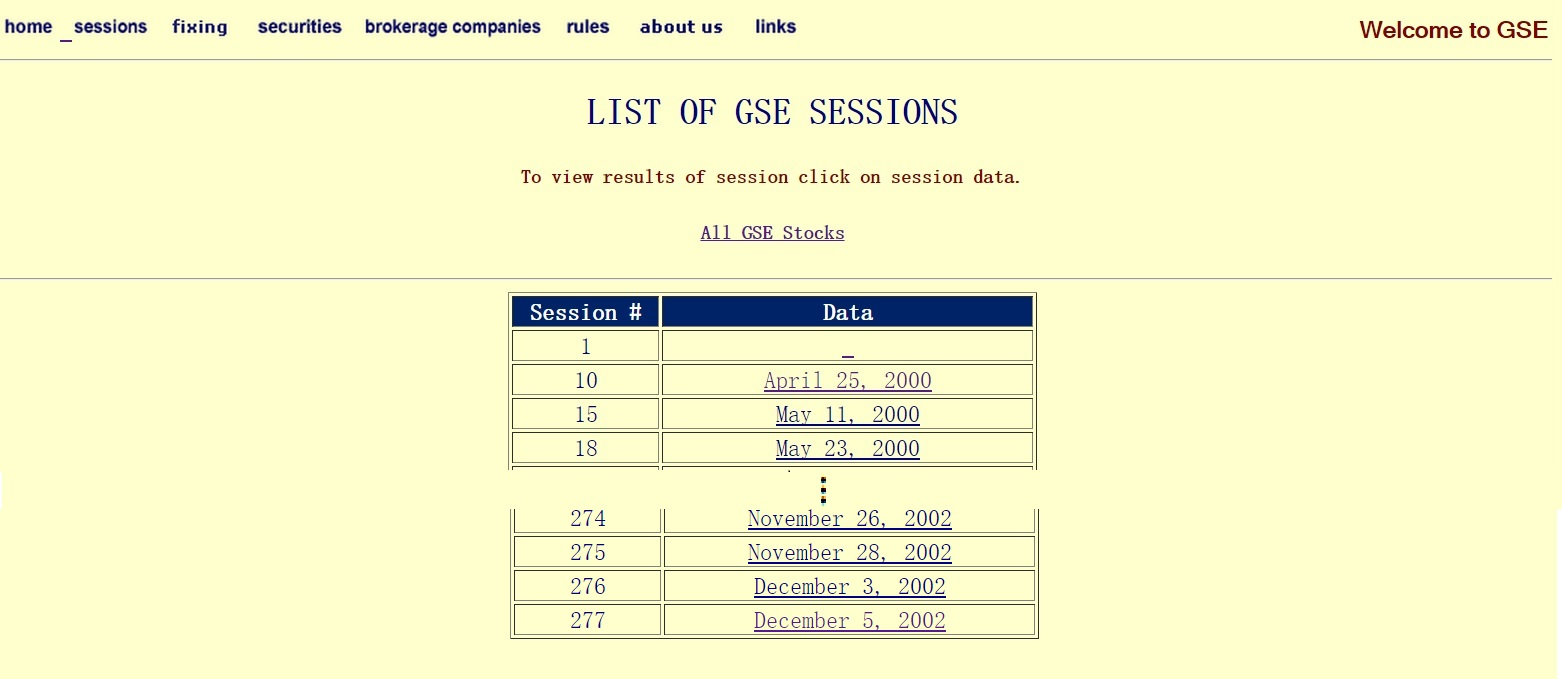
\includegraphics[width=6.3in, height=3.2in]{images/sessions.jpg}
\caption{GSE data taken on Jan. 14th, 2015 for ``all'' sessions of trading. However, as we see, the list is very uncomprehensive and the list ends on Dec. 5th, 2002. Therefore, it is very difficult for potential investors to follow the market, since daily update of stock trade results are not available. In addition, notice again that no direct download link is available.}
\label{fig:sessions}
\end{figure}

Fortunately, all data on the website are organized in an XML-accessible way. Therefore, we can use \texttt{R} and \texttt{XML} package to write a downloader of the stock data.

\section{Introducing GeorgianStockParser Package}
\label{sec:package}

\subsection{Downloading Functions}
\label{subsec:functions}
There are four downloading functions: \texttt{download.stockIDs}, \texttt{download.single.stock.trade}, \texttt{download.multi.stock.trade}, and \texttt{download.all.stock.trade}.

\texttt{download.stockIDs} scans the data from the webpage (see Figure \ref{fig:stocks}) and returns a data frame containing all the stock symbols and corresponding company names. The parameter \texttt{export} specifies whether to export the data frame to an \texttt{.csv} file (\texttt{export} defaultly set to \texttt{FALSE}).

\begin{Schunk}
\begin{Sinput}
> library(GeorgianStockParser)
> stocks <- download.stockIDs(export = FALSE)
> head(stocks)
\end{Sinput}
\begin{Soutput}
  Trade Symbol              Name of JSC
1      $GLC01H Georgian Leasing Company
2         AEST                   Telasi
3         AGVQ           Akhmeta Winery
4         AKAT                    Aqati
5          AMA                  Amaltea
6         AMCE          Amtse (Tbilisi)
\end{Soutput}
\begin{Sinput}
> tail(stocks)
\end{Sinput}
\begin{Soutput}
    Trade Symbol        Name of JSC
124         UNVR          Universal
125         UQQS Uksovadi Ksovilebi
126          UTC     United Telecom
127         VAZI            Vaziani
128         VERE        Laguna Vere
129         WINE     Teliani Valley
\end{Soutput}
\end{Schunk}

\texttt{download.single.stock.trade} scans the data from the webpage (see Figure \ref{fig:AGVQ}) and returns a data frame containing all the trade results of the stock. The parameter \texttt{ID} takes a character string of the stock symbol we want trade results of, and \texttt{export} means the same as previously.

\begin{Schunk}
\begin{Sinput}
> AGVQ <- download.single.stock.trade(ID = "AGVQ", export = FALSE)
> tail(AGVQ)
\end{Sinput}
\begin{Soutput}
   Session       Date Trades Min. price Max.price Weighted avg. price
6      664 2006-10-17      1       1.50      1.50                1.50
7      668 2006-10-31      1       1.50      1.50                1.50
8      673 2006-11-16      1       1.50      1.50                1.50
9      682 2006-12-21      1       1.80      1.80                1.80
10     683 2006-12-26      1       1.25      1.25                1.25
11     684 2006-12-28      1       1.00      1.00                1.00
   Weighted closing price Volume in Securities Volume in GEL
6                      NA                 4530        6795.0
7                      NA                 2069        3103.5
8                    1.50                  667        1000.5
9                    1.80                 1669        3004.2
10                   1.25                 3200        4000.0
11                   1.00                 4461        4461.0
\end{Soutput}
\end{Schunk}

\texttt{download.multi.stock.trade} scans the data from the website and returns a data frame containing trade results of multiple stocks we specify. The parameter \texttt{ID} takes a data frame of the stock symbols we want trade results of, and \texttt{export} means the same as previously.

\begin{Schunk}
\begin{Sinput}
> multiID <- data.frame(ID = c("AGVQ", "VAZI"))
> multi <- download.multi.stock.trade(ID = multiID, export = FALSE)
> head(multi)
\end{Sinput}
\begin{Soutput}
    ID Session       Date Trades Min. price Max.price Weighted avg. price
1 AGVQ     302 2003-03-11      1       0.05      0.05                0.05
2 AGVQ     330 2003-06-17      3       0.10      0.10                0.10
3 AGVQ     332 2003-06-24      6       0.10      0.10                0.10
4 AGVQ     662 2006-10-10      1       0.25      0.25                0.25
5 AGVQ     663 2006-10-12      1       1.50      1.50                1.50
6 AGVQ     664 2006-10-17      1       1.50      1.50                1.50
  Weighted closing price Volume in Securities Volume in GEL
1                     NA                 6676        333.80
2                     NA                13783       1378.30
3                     NA               110564      11056.40
4                     NA                16691       4172.75
5                     NA                 4500       6750.00
6                     NA                 4530       6795.00
\end{Soutput}
\begin{Sinput}
> tail(multi)
\end{Sinput}
\begin{Soutput}
     ID Session       Date Trades Min. price Max.price Weighted avg. price
12 VAZI     304 2003-03-18      5        0.3       0.3                 0.3
13 VAZI     319 2003-05-08      4        0.3       0.3                 0.3
14 VAZI     489 2005-01-13      2        3.0       3.0                 3.0
15 VAZI     540 2005-07-26      5        3.0       3.0                 3.0
16 VAZI     558 2005-09-27      1        3.0       3.0                 3.0
17 VAZI     638 2006-07-13      1        2.0       2.0                 2.0
   Weighted closing price Volume in Securities Volume in GEL
12                     NA                 9149        2744.7
13                     NA                 9149        2744.7
14                     NA                 1830        5490.0
15                     NA                 1830        5490.0
16                     NA                   11          33.0
17                     NA                 2872        5744.0
\end{Soutput}
\end{Schunk}

\texttt{download.all.stock.trade} scans the data from the website and returns a data frame containing all trade results of all registered stocks. The parameter \texttt{export} means the same as previously. This function can create a good sample for time-series analysis on Georgian stock market. All analyzing functions and results will be based on the \texttt{all} data set generated by this function.

\begin{Schunk}
\begin{Sinput}
> ## all <- download.all.stock.trade(export = FALSE)
> ## tail(all)
> ## dim(all) ## the first number is the current number of trades that ever happened
\end{Sinput}
\end{Schunk}

There is still yet one more downloading function to add, which is \texttt{daily.update}. \texttt{daily.update} should take a \texttt{date} parameter of \texttt{Date} type, and download all the trade results that happen on that specified date. This function should be used as a survey tool of what happened after a specific event, say Russian-Georgian War in 2008. Or it can be used as a data set update function, since we don't want to slowly run \texttt{download.all.stock.trade} every time. The function can be most easily created by going into the ``All Session Report'' on GSE website, but since the website only contains data before 2003, we have to come up with a new way. Due to limited time availability on this project, I will not create this function, since with the \texttt{all} data set we can already start the analysis.

\section{Conclusion}

In this paper, ...


\end{document}
